\usetikzlibrary{arrows}
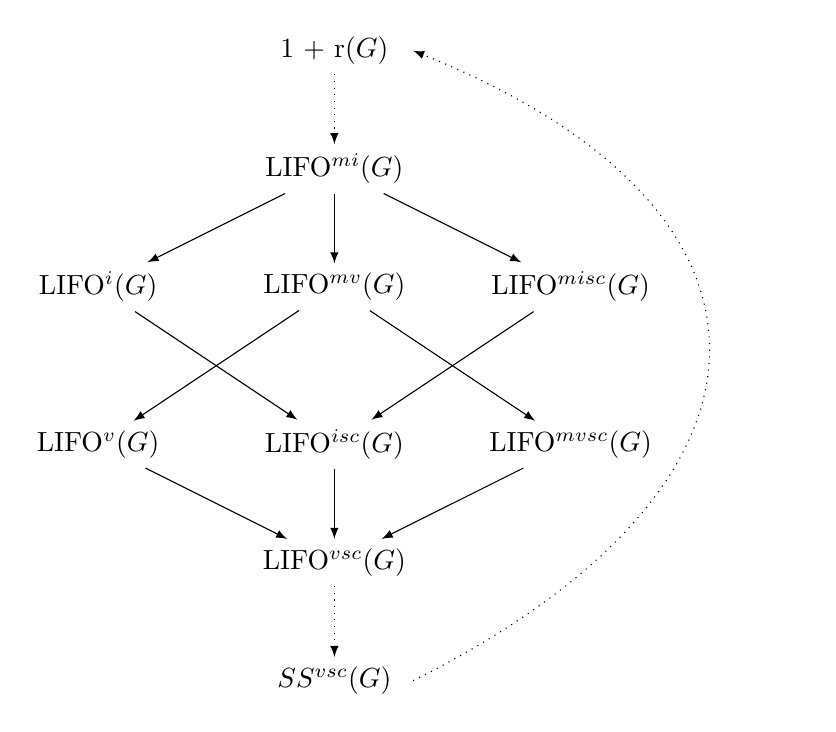
\begin{tikzpicture}

\node (v1) at (0,0) {LIFO$^{mi}(G)$};
\node (v2) at (-3,-1.5) {LIFO$^{i}(G)$};
\node (v3) at (0,-1.5) {LIFO$^{mv}(G)$};
\node (v4) at (3,-1.5) {LIFO$^{misc}(G)$};
\draw [-latex] (v1) edge (v2);
\draw [-latex] (v1) edge (v3);
\draw [-latex] (v1) edge (v4);
\node (v6) at (-3,-3.5) {LIFO$^{v}(G)$};
\node (v5) at (0,-3.5) {LIFO$^{isc}(G)$};
\node (v7) at (3,-3.5) {LIFO$^{mvsc}(G)$};
\draw [-latex] (v2) edge (v5);
\draw [-latex] (v4) edge (v5);
\draw [-latex] (v3) edge (v6);
\draw [-latex] (v3) edge (v7);
\node (v8) at (0,-5) {LIFO$^{vsc}(G)$};
\draw [-latex] (v6) edge (v8);
\draw [-latex] (v7) edge (v8);
\draw [-latex] (v5) edge (v8);
\node (v9) at (0,1.5) {1 + r($G$)};
\draw [dotted, -latex] (v9) edge (v1);
\node (v10) at (0,-6.5) {$SS^{vsc}(G)$};
\draw [dotted, -latex] (v8) edge (v10);

\draw [dotted, -latex](1,-6.5) .. controls (6,-4) and (6,-0.5) .. (1,1.5);
\end{tikzpicture}